An \textit{n}-body simulation is a simulation of \textit{n} number of bodies, as
the name would suggest. We simulate the interactions between all of the
\textit{n} bodies. The bodies are located in a three-dimensional space. In each
tick the simulation calculates the every body (or pointmass) interaction, with
all the other pointmasses in the simulation. The interaction can vary, with
gravitational attraction being the simplest.

If we were to compute the interaction for each body at each step of the
simulation for some $\Delta$ time, naively, we would have a running time of
$O(n^2)$, and since the simulation could be expected to work on very large
values of $n$, as well as the interaction might be timeconsuming to calculate,
it will end up being slow. Therefore we implement a clustered version instead
inspired by the barnes hut algorithm. The idea is that by defining clusters of
bodies we can approximate a region of points, as a single point. The clustered
version is tree-based meaning that we store each pointmass in a tree, and based
on some threshold $\theta$ we determine when we should calculate the interaction
between the actual pointmasses, and when to calculate it for the clustered
representation.
\subsection{Naive simulation}
The naive simulation is to simply put it, apply the sum of all forces from all
other pointmasses to all pointmasses:         \\
$B: \mbox{Bodies},$                           \\
$n: |B|,$                                     \\
$b^i_m: \mbox{mass of } b^i,$                 \\
$b^i_p: \mbox{position of } b^i \mbox{represented as a $d$-dimensional vector}$\\
$b^i_f: \mbox{force of } b^i,$                \\
$\Delta t: \mbox{Change in time},$                \\
$r(a, b): b_p - a_p, \mbox{position difference as a $d$-dimensional vector}$\\
$F(a, b): G \cdot a_m \cdot b_m \cdot |r(b - a)|^2 \cdot (\frac{1}{|r|} \cdot r)$
$$\forall b \in B (\forall a \in B \backslash \left\{ b^i\right\} | b^i_F = \sum F(b^i, a^i))$$

We then apply the force as acceleration scaled with $\Delta t$ on velocity
times $\Delta t$ and apply the velocity as a change in position to each
pointmass in the simulation.

This ultimately result in a computation of $O(n^2)$.
If we try and parallelize this computation we can do this with a work and span of \red{<INSERT>}.

\subsection{Barnes-Hut simulation}
To perform this clustered \textit{n}-body simulation, we make use of the
Barnes-Hut algorithm\cite{BH-algo}. In Barnes-Hut we can use an octree for 3D
or a quadtree for 2D simulation. This is typically done since the space
containing these bodies can be subdivided into these types of trees. A 2D
exmaple of this can be seen in figure \ref{fig:subdivision}.

\begin{Figure}
  \centering
  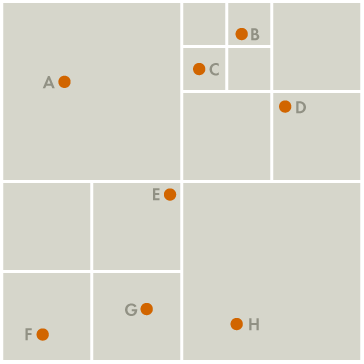
\includegraphics[width=0.30\textwidth]{assests/example-space}
  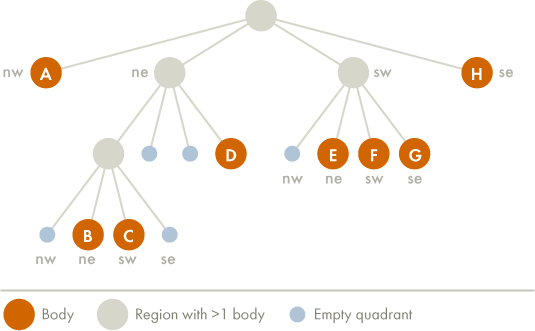
\includegraphics[width=0.65\textwidth]{assests/example-tree}
  \captionof{figure}{A sample space subdivided into regions, with each region
    containing 1 body. The quadtree created from this 2D space can also be seen.
  Figure is courtesy by \url{arborjs.org/docs/barnes-hut}}
  \label{fig:subdivision}
\end{Figure}

We then
